\documentclass[12pt,a4paper]{report}

% ===================== PACKAGES =====================
\usepackage[a4paper,margin=1in]{geometry}
\usepackage{fontspec}
\IfFontExistsTF{Noto Serif}
    {\setmainfont{Noto Serif}}
    {\setmainfont{Times New Roman}}
\usepackage{setspace}
\usepackage{graphicx}
\usepackage{float}
\usepackage{booktabs}
\usepackage{array}
\usepackage{longtable}
\usepackage{tabularx}
\usepackage{multirow}
\usepackage{amsmath,amssymb}
\usepackage{enumitem}
\usepackage{xcolor}
\usepackage{hyperref}
\usepackage{caption}
\usepackage{tikz}
\usetikzlibrary{arrows.meta,positioning,calc,fit,backgrounds,shapes.geometric}

\definecolor{paperblue}{RGB}{70,105,150}
\definecolor{paperorange}{RGB}{215,120,55}
\definecolor{papergreen}{RGB}{110,150,110}
\definecolor{softblue}{RGB}{226,236,248}
\definecolor{softorange}{RGB}{252,232,215}
\definecolor{softgreen}{RGB}{229,241,226}
\definecolor{darkgray}{RGB}{45,45,45}

\hypersetup{
    colorlinks=true,
    linkcolor=black,
    urlcolor=blue,
    citecolor=black
}

\onehalfspacing
\sloppy
\setcounter{secnumdepth}{3}
\setcounter{tocdepth}{3}

\newcolumntype{Y}{>{\raggedright\arraybackslash}X}
\newcolumntype{C}{>{\centering\arraybackslash}X}
\newcommand{\code}[1]{\texttt{#1}}
\newcommand{\artifactpath}[1]{{\footnotesize\path{#1}}}
\newcommand{\metric}[1]{\textbf{#1}}
\newcommand{\safeincludegraphics}[2][]{%
    \IfFileExists{#2}{%
        \includegraphics[#1]{#2}%
    }{%
        \fbox{\parbox{0.86\textwidth}{\centering Missing figure: \code{#2}}}%
    }%
}

\begin{document}

% ===================== COVER PAGE 1 =====================
\pagenumbering{roman}
\begin{titlepage}
    \centering
    \vspace*{0.7cm}
    {\Large\bfseries VIETNAM GENERAL CONFEDERATION OF LABOUR\\[0.3cm]}
    {\Large\bfseries TON DUC THANG UNIVERSITY\\[0.3cm]}
    {\Large\bfseries FACULTY OF INFORMATION TECHNOLOGY\\[0.8cm]}

    \safeincludegraphics[width=0.22\textwidth]{figures/tdtu.png}\\[1.2cm]

    {\Large\bfseries GROUP 11\\[1.4cm]}
    {\Huge\bfseries ENDTERM REPORT ON\\[0.4cm] DATA MINING\\[1.8cm]}

    {\Huge\bfseries FIRE AND SMOKE DETECTION\\[0.4cm]}
    {\Huge\bfseries USING COMPUTER VISION\\[1.8cm]}

    {\Large\bfseries HO CHI MINH CITY, 2026}
\end{titlepage}

% ===================== COVER PAGE 2 =====================
\begin{titlepage}
    \centering
    \vspace*{0.7cm}
    {\Large\bfseries VIETNAM GENERAL CONFEDERATION OF LABOUR\\[0.3cm]}
    {\Large\bfseries TON DUC THANG UNIVERSITY\\[0.3cm]}
    {\Large\bfseries FACULTY OF INFORMATION TECHNOLOGY\\[0.8cm]}

    \safeincludegraphics[width=0.20\textwidth]{figures/tdtu.png}\\[0.9cm]

    {\Large\bfseries GROUP 11\\[1.1cm]}
    {\Huge\bfseries ENDTERM REPORT ON\\[0.4cm] DATA MINING\\[1.1cm]}

    {\large Advised by\\[0.3cm]}
    {\large Dr. Hoang Anh\\[0.7cm]}

    {\Huge\bfseries FIRE AND SMOKE DETECTION\\[0.4cm]}
    {\Huge\bfseries USING COMPUTER VISION\\[1.5cm]}

    {\Large\bfseries HO CHI MINH CITY, 2026}
\end{titlepage}

% ===================== GROUP MEMBERS =====================
\chapter*{Table of Group Members}
\addcontentsline{toc}{chapter}{Table of Group Members}
\begin{center}
\begin{tabular}{ll}
\toprule
\textbf{Name} & \textbf{Student ID} \\
\midrule
Đỗ Tâm Phúc & 523H0078 \\
Phạm Ngọc Dương & 523H0016 \\
Trần Gia Lạc & 523H0154 \\
Huỳnh Mạnh Phát & 523H0167 \\
Phạm Nguyễn Thanh Phong & 523H0169 \\
Hoàng Xuân Thành & 523H0178 \\
\bottomrule
\end{tabular}
\end{center}

\tableofcontents
\listoffigures
\listoftables

% ===================== ABBREVIATIONS =====================
\chapter*{Abbreviations}
\addcontentsline{toc}{chapter}{Abbreviations}
\begin{center}
\begin{tabular}{ll}
\toprule
\textbf{Abbreviation} & \textbf{Meaning} \\
\midrule
AI & Artificial Intelligence \\
AP & Average Precision \\
COCO & Common Objects in Context annotation format \\
CV & Computer Vision \\
dHash & Difference perceptual hash \\
EDA & Exploratory Data Analysis \\
FN & False Negative \\
FP & False Positive \\
GPU & Graphics Processing Unit \\
IoU & Intersection over Union \\
mAP & mean Average Precision \\
NMS & Non-Maximum Suppression \\
QA & Quality Assurance \\
SAHI & Slicing Aided Hyper Inference \\
TP & True Positive \\
YOLO & You Only Look Once object detector family \\
\bottomrule
\end{tabular}
\end{center}

\clearpage
\pagenumbering{arabic}

\begin{center}
    {\Large\bfseries FIRE AND SMOKE DETECTION USING COMPUTER VISION}
\end{center}

% ===================== ABSTRACT =====================
\chapter*{Executive Summary}
\addcontentsline{toc}{chapter}{Executive Summary}
This report presents a complete Data Mining and Computer Vision pipeline for detecting fire and smoke in diverse Vietnamese visual contexts. The project does not simply fine-tune an existing detector on a clean benchmark. Instead, the main contribution is the construction of a traceable end-to-end workflow: noisy multi-source data collection, custom segmentation labeling, label quality control, duplicate and near-duplicate removal, group-aware dataset design, train-only slicing for rare small-object cases, YOLO11x detection training, and systematic error analysis.

The final model direction is a single-class YOLO11x detector named \code{fire\_smoke}. Although the original labels are built as segmentation masks, the deployment-oriented model is formulated as detection because an alerting system needs fast and stable bounding-box outputs more than pixel-perfect masks. The training was conducted on rented NVIDIA L4 GPU infrastructure, with an experimental cost of approximately \(1{,}000{,}000\) VND. This cost produced real checkpoints, training curves, validation metrics, full-image test metrics, sliced inference ablations, qualitative prediction samples, and a local Streamlit interface for testing inference with the packaged Stage 1/2 model artifact.

The best Stage 2 validation result reached \metric{mAP@50 = 0.454} and \metric{mAP@50:95 = 0.262}. On the original full-image test split, the same checkpoint achieved \metric{Precision = 0.552}, \metric{Recall = 0.430}, \metric{mAP@50 = 0.421}, and \metric{mAP@50:95 = 0.240}. These metrics are below the original target of mAP@50 \(\geq 0.70\), but they are substantially more informative than the earlier sliced-only result. The sliced inference ablation reached only mAP@50 \(=0.152\), showing that the current slicing and merging protocol is not yet tuned. The report therefore emphasizes an academically honest conclusion: the current model is not deployment-ready, but the dataset, pipeline, and error analysis establish a strong foundation for active learning, relabeling, hard-negative expansion, and threshold/NMS optimization.

% ===================== CHAPTER 1 =====================
\chapter{Introduction}
\section{Problem Context}
Early fire and smoke detection is a safety-critical Computer Vision problem. The objective is to detect visual indicators of fire or smoke from still images or camera streams before an incident escalates. In contrast to many conventional object detection tasks, fire and smoke do not have stable shapes, rigid contours, or consistent texture. Fire changes rapidly over time, smoke is semi-transparent, and early-stage ignition can occupy only a tiny area of the frame.

This project focuses on contexts that are visually relevant to Vietnam: residential alleyways, dense urban backgrounds, low-light footage, small flame spots, smoke mixed with haze, and hard negative scenes such as lamps, candles, reflections, and warm-colored lighting. These scenarios are deliberately harder than clean forest-fire or large-flame examples.

\section{Why This is a Data Mining Project}
The central problem is not only model selection. A high-capacity detector cannot perform well if the data are noisy, duplicated, mislabeled, or evaluation splits leak near-identical frames. The project therefore follows the Data Mining lifecycle:

\begin{enumerate}
    \item Collect raw visual data from heterogeneous sources.
    \item Organize data into meaningful semantic groups.
    \item Build segmentation annotations where no original masks existed.
    \item Audit labels and remove corrupted or irrelevant samples.
    \item Detect exact and perceptual duplicates.
    \item Build deterministic train/validation/test splits.
    \item Train YOLO11x using a two-stage strategy.
    \item Analyze metrics by dataset group and failure mode.
\end{enumerate}

\section{Key Contributions}
The report should be evaluated not only by the final mAP value, but also by the engineering work required to produce a valid experimental setting. The main contributions are:

\begin{itemize}
    \item \textbf{Multi-source data collection:} Images were collected and selected from Kaggle, Google Images, self-curated Vietnamese contexts, hard negatives, and ambient null scenes.
    \item \textbf{Custom segmentation labeling:} The original public data did not provide segmentation masks. Fire and smoke regions were manually annotated and quality checked.
    \item \textbf{Data quality control:} The pipeline detects corrupted files, empty labels, invalid coordinates, exact duplicates, and near-duplicate frames.
    \item \textbf{Leakage-aware splitting:} Splits are performed at source-image level before slicing to avoid inflated validation scores.
    \item \textbf{Compute-backed training:} The YOLO11x detector was trained and fine-tuned on rented NVIDIA L4 GPU resources, costing approximately \(1{,}000{,}000\) VND.
    \item \textbf{Honest error analysis:} The report explains why the metrics are below the original target and identifies concrete improvement directions.
\end{itemize}

\section{System Objective}
The original technical target was to approach mAP@50 \(\geq 0.70\) for a one-class fire/smoke detector. The achieved result is lower, but the system still satisfies several important research and engineering objectives:

\begin{itemize}
    \item a reproducible dataset preparation pipeline;
    \item a curated dataset with 13,896 images and 28,279 annotated objects after deduplication;
    \item a two-stage YOLO11x training workflow;
    \item validation, full-image test, per-group, and sliced inference evaluation artifacts;
    \item a published Hugging Face model artifact and a local Streamlit inference UI for checkpoint testing;
    \item a clear diagnosis of false negatives, hard-negative false positives, and sliced inference weaknesses.
\end{itemize}

% ===================== CHAPTER 2 =====================
\chapter{Data Collection and Annotation}
\section{Data Sources}
The dataset was designed to avoid a common failure in fire detection research: training on obvious large fires and then failing on early-stage or ambiguous camera scenes. Table~\ref{tab:data-sources} summarizes the data sources.

\begin{table}[H]
\centering
\caption{Data sources and their roles}
\label{tab:data-sources}
\begin{tabularx}{\textwidth}{p{0.22\textwidth}YY}
\toprule
\textbf{Source} & \textbf{Contribution} & \textbf{Main Issues} \\
\midrule
Kaggle images & Diverse public fire/smoke examples. & Images only; no segmentation masks. \\
Google Images & Civilian scenes, small fire, faint smoke, local contexts. & Watermarks, duplicates, inconsistent quality. \\
Self-curated data & Vietnamese alleyways and residential contexts. & Requires normalization and manual labeling. \\
Hard negatives & Lamps, candles, reflections, warm lighting, non-fire smoke-like patterns. & Must remain unlabeled to teach rejection. \\
Ambient null images & Normal background frames without incidents. & Important for reducing false alarms. \\
\bottomrule
\end{tabularx}
\end{table}

\section{Dataset Availability}
The prepared dataset is published on Hugging Face at:

\begin{center}
\url{https://huggingface.co/datasets/thanhhoangnvbg/fire-vn-yolo11seg-v1}
\end{center}

The submission package does not include the local dataset files because they are large and can be regenerated from the public dataset repository using the provided preparation scripts. This keeps the submitted archive focused on the report, code, and reproducible processing pipeline.

\section{Model Artifact and Inference Interface}
The Stage 1 and Stage 2 training outputs are packaged separately from the source code because checkpoint files are large. The model artifact is published on Hugging Face at:

\begin{center}
\url{https://huggingface.co/thanhhoangnvbg/fire-detection-yolo11-stage12}
\end{center}

The downloadable artifact is \code{model\_artifacts\_stage12\_complete.tar.gz}. After extraction, the default inference checkpoint is the Stage 2 fine-tuned model:

\begin{center}
\artifactpath{weights/fire-detection-yolo11-stage12/runs/final/yolo11x_detect_fire_smoke_l4_finetune/weights/best.pt}
\end{center}

For practical testing, the project includes a Streamlit interface in \code{app.py}. The interface loads the checkpoint, accepts uploaded images or bundled sample images, allows confidence, IoU, image-size, and device settings to be adjusted, and displays both the original image and the annotated prediction output. This UI is intended as a reproducible inference test tool, not as a production monitoring system.

\begin{figure}[H]
\centering
\safeincludegraphics[width=0.98\textwidth]{figures/streamlit_inference_ui.png}
\caption{Streamlit inference interface for testing the packaged Stage 2 YOLO11 checkpoint on \code{Chay-Rung-3.jpg}.}
\label{fig:streamlit-inference-ui}
\end{figure}

\section{Dataset Group Design}
Instead of treating all images as a flat pool, the dataset is organized into five groups. This design makes it possible to diagnose exactly where the model succeeds or fails.

\begin{table}[H]
\centering
\caption{Dataset groups}
\label{tab:dataset-groups}
\begin{tabularx}{\textwidth}{p{0.12\textwidth}p{0.24\textwidth}Y}
\toprule
\textbf{Group} & \textbf{Name} & \textbf{Role} \\
\midrule
g01 & \code{positive\_standard} & Main positive data with visible fire/smoke instances. \\
g02 & \code{alley\_context} & Difficult Vietnamese alley/residential scenes. \\
g03 & \code{hard\_negative} & Non-fire confusing samples such as lamps and reflections. \\
g04 & \code{sahi\_small\_objects} & Small fire/smoke objects that require special slicing. \\
g05 & \code{ambient\_null} & Normal background images used to reduce false alarms. \\
\bottomrule
\end{tabularx}
\end{table}

\section{Manual Segmentation Annotation}
A major effort of the project is the creation of segmentation annotations. Many source images had no pixel-level labels. The team therefore annotated visible fire and smoke regions with polygon masks. This is much more expensive than image-level classification because annotators must decide where the flame or smoke boundary begins and ends.

The annotation protocol follows these principles:

\begin{itemize}
    \item label only visible fire/smoke regions, not the entire bright area;
    \item do not label watermarks, timestamps, camera overlays, or unrelated text;
    \item label partially occluded fire only where it is visible;
    \item label smoke only when it has enough visual structure to distinguish it from background haze;
    \item keep hard negatives unlabeled even if they contain fire-like colors;
    \item export verified data to COCO segmentation and then convert it to YOLO formats.
\end{itemize}

\section{Why the Labeling Work Matters}
The final metric is not high, but the labeling work remains valuable. Without segmentation labels, the model would either learn only image-level correlations or rely on noisy bounding boxes. Segmentation masks preserve shape information and allow a clean conversion into detection boxes. This makes the final one-class detector more grounded in actual fire/smoke regions.

The practical challenge is that fire and smoke are not rigid objects. Flame boundaries are fuzzy and smoke is semi-transparent. Too-wide masks make the model learn background; too-tight masks reduce recall on diffuse smoke and spreading fire. The labeling process therefore represents a trade-off between geometric precision and practical detection stability.

\section{Annotation Quality Limitation}
Although the report documents the annotation protocol, the current artifact set does not contain a quantitative annotation-quality study. This is a real limitation. With six members participating in data collection and labeling, label inconsistency is a plausible source of noise. Examples include different interpretations of faint smoke, inconsistent treatment of reflections, and different polygon tightness around flame boundaries.

The missing measurements are:

\begin{itemize}
    \item \textbf{Inter-annotator agreement:} A shared subset should be labeled by at least two annotators and compared using mask IoU, box IoU, or object-level F1.
    \item \textbf{Label error rate:} A random audit sample should be reviewed after export to estimate missing labels, wrong labels, overly wide masks, and false positive labels.
    \item \textbf{Boundary consistency:} Smoke and flame masks should be evaluated separately because smoke has more subjective boundaries than flame.
\end{itemize}

Because these measurements were not completed, the report should not overclaim that the labels are fully consistent. A more accurate conclusion is that the labels were created and QA-checked procedurally, but their statistical reliability remains an open experimental issue.

% ===================== CHAPTER 3 =====================
\chapter{Exploratory Data Analysis}
\section{Final Dataset Overview}
After preprocessing and near-duplicate removal, the final dataset contains 13,896 images and 28,279 annotated objects. Table~\ref{tab:dataset-overview} summarizes the final state.

\begin{table}[H]
\centering
\caption{Final dataset overview after deduplication}
\label{tab:dataset-overview}
\begin{tabular}{lr}
\toprule
\textbf{Statistic} & \textbf{Value} \\
\midrule
Total images & 13,896 \\
Total segmentation objects & 28,279 \\
Background images & 4,099 \\
Background ratio & 29.50\% \\
Smoke objects & 12,356 \\
Fire objects & 15,923 \\
\bottomrule
\end{tabular}
\end{table}

\section{Before and After Deduplication}
Deduplication intentionally reduces the apparent amount of data. This is not a weakness: it prevents optimistic metrics caused by nearly identical frames appearing across splits.

\begin{table}[H]
\centering
\caption{Dataset size before and after near-duplicate removal}
\label{tab:dedupe-impact}
\begin{tabular}{lrrp{0.36\textwidth}}
\toprule
\textbf{Stage} & \textbf{Images} & \textbf{Objects} & \textbf{Interpretation} \\
\midrule
Before near-dedupe & 15,615 & 31,134 & Detection-level dataset before removing near-duplicate scenes. \\
After near-dedupe & 13,896 & 28,279 & Final dataset used for training/evaluation. \\
Change & -1,719 & -2,855 & Reduces repeated scenes and duplicate object evidence. \\
\bottomrule
\end{tabular}
\end{table}

At source-image level, perceptual deduplication detected 1,095 near-duplicate clusters and removed 1,649 source images. Most removals came from \code{g01 positive\_standard}, where repeated frames from the same event were common.

\begin{figure}[H]
\centering
\safeincludegraphics[width=0.86\textwidth]{data_audit_deduped/near_duplicates/near_duplicate_cluster_001.jpg}
\caption{Example near-duplicate cluster found by perceptual hashing.}
\label{fig:near-duplicate}
\end{figure}

\section{Split Distribution}
The final train/validation/test split is shown in Table~\ref{tab:split-distribution}. Validation and test are kept as full images, while slicing is applied only to selected training groups.

\begin{table}[H]
\centering
\caption{Distribution by split}
\label{tab:split-distribution}
\begin{tabular}{lrrr}
\toprule
\textbf{Split} & \textbf{Images} & \textbf{Objects} & \textbf{Background Images} \\
\midrule
Train & 12,322 & 25,086 & 3,628 \\
Validation & 841 & 1,724 & 252 \\
Test & 733 & 1,469 & 219 \\
\bottomrule
\end{tabular}
\end{table}

\begin{figure}[H]
\centering
\safeincludegraphics[width=0.86\textwidth]{data_audit_deduped/figures/images_by_split_group.png}
\caption{Images by split and group.}
\label{fig:images-split-group}
\end{figure}

\begin{figure}[H]
\centering
\safeincludegraphics[width=0.86\textwidth]{data_audit_deduped/figures/objects_by_split_group.png}
\caption{Objects by split and group.}
\label{fig:objects-split-group}
\end{figure}

\section{Group Distribution}
\begin{longtable}{llrrr}
\caption{Group-level split distribution}\label{tab:group-distribution}\\
\toprule
\textbf{Split} & \textbf{Group} & \textbf{Images} & \textbf{Objects} & \textbf{Background Ratio} \\
\midrule
\endfirsthead
\toprule
\textbf{Split} & \textbf{Group} & \textbf{Images} & \textbf{Objects} & \textbf{Background Ratio} \\
\midrule
\endhead
Train & g01 positive\_standard & 6,552 & 18,479 & 0.0000 \\
Train & g02 alley\_context & 1,711 & 4,498 & 0.1099 \\
Train & g03 hard\_negative & 555 & 0 & 1.0000 \\
Train & g04 sahi\_small\_objects & 612 & 2,086 & 0.0000 \\
Train & g05 ambient\_null & 2,892 & 23 & 0.9976 \\
Validation & g01 positive\_standard & 527 & 1,511 & 0.0000 \\
Validation & g02 alley\_context & 42 & 105 & 0.0000 \\
Validation & g03 hard\_negative & 19 & 0 & 1.0000 \\
Validation & g04 sahi\_small\_objects & 20 & 108 & 0.0000 \\
Validation & g05 ambient\_null & 233 & 0 & 1.0000 \\
Test & g01 positive\_standard & 452 & 1,245 & 0.0000 \\
Test & g02 alley\_context & 42 & 132 & 0.0000 \\
Test & g03 hard\_negative & 19 & 0 & 1.0000 \\
Test & g04 sahi\_small\_objects & 20 & 92 & 0.0000 \\
Test & g05 ambient\_null & 200 & 0 & 1.0000 \\
\bottomrule
\end{longtable}

\section{Visual and Statistical Patterns}
\begin{figure}[H]
\centering
\safeincludegraphics[width=0.76\textwidth]{data_audit_deduped/figures/class_distribution.png}
\caption{Class distribution of fire and smoke objects.}
\label{fig:class-distribution}
\end{figure}

\begin{figure}[H]
\centering
\safeincludegraphics[width=0.78\textwidth]{data_audit_deduped/figures/object_area_distribution.png}
\caption{Object area distribution.}
\label{fig:area-distribution}
\end{figure}

\begin{figure}[H]
\centering
\safeincludegraphics[width=0.78\textwidth]{data_audit_deduped/figures/object_width_height_scatter.png}
\caption{Object width-height scatter.}
\label{fig:wh-scatter}
\end{figure}

The EDA highlights three important points. First, \code{g01} remains the dominant group, so its false negatives strongly influence the overall metric. Second, \code{g03} and \code{g05} contain no positive labels but are essential for reducing false alarms. Third, \code{g04} has fewer images but a high object density, making it important for early-stage small-fire detection.

% ===================== CHAPTER 4 =====================
\chapter{Data Preprocessing}
\section{Pipeline Overview}
The preprocessing pipeline is implemented by project scripts such as \code{prepare\_yolo11\_seg\_dataset.py}, \code{prepare\_yolo11\_detect\_dataset.py}, and \code{generate\_yolo11\_data\_report.py}. Figure~\ref{fig:pipeline} summarizes the workflow.

\begin{figure}[H]
\centering
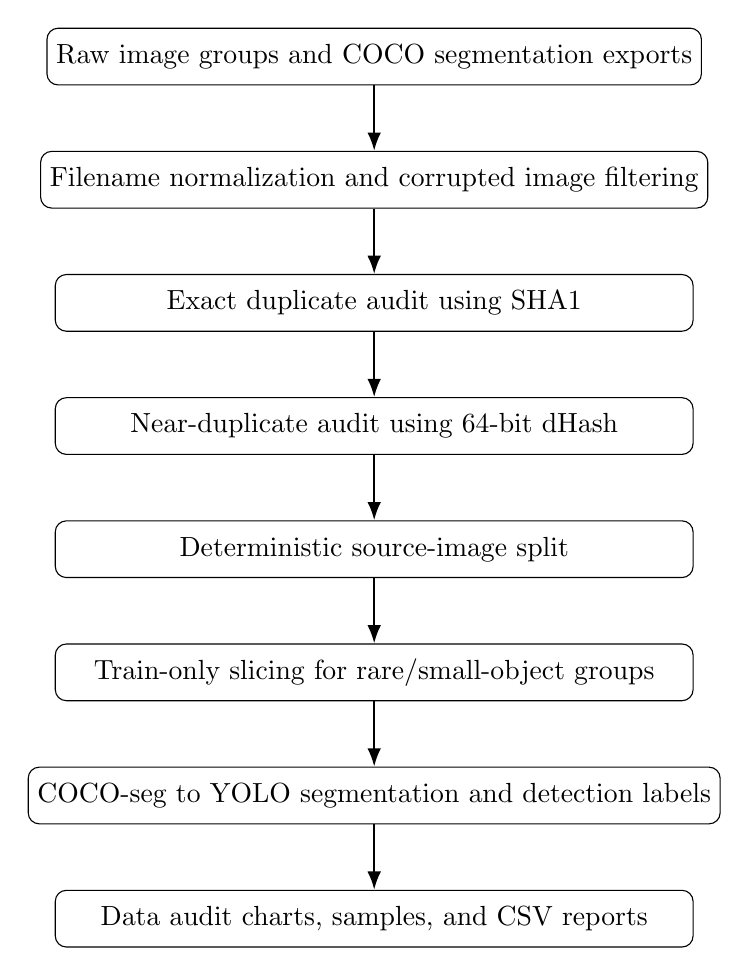
\begin{tikzpicture}[
    node distance=0.83cm,
    process/.style={rectangle, rounded corners, draw, align=center, minimum width=8.1cm, minimum height=0.72cm},
    arrow/.style={-{Latex}, thick}
]
\node[process] (raw) {Raw image groups and COCO segmentation exports};
\node[process, below=of raw] (normalize) {Filename normalization and corrupted image filtering};
\node[process, below=of normalize] (hash) {Exact duplicate audit using SHA1};
\node[process, below=of hash] (near) {Near-duplicate audit using 64-bit dHash};
\node[process, below=of near] (split) {Deterministic source-image split};
\node[process, below=of split] (slice) {Train-only slicing for rare/small-object groups};
\node[process, below=of slice] (convert) {COCO-seg to YOLO segmentation and detection labels};
\node[process, below=of convert] (audit) {Data audit charts, samples, and CSV reports};
\draw[arrow] (raw) -- (normalize);
\draw[arrow] (normalize) -- (hash);
\draw[arrow] (hash) -- (near);
\draw[arrow] (near) -- (split);
\draw[arrow] (split) -- (slice);
\draw[arrow] (slice) -- (convert);
\draw[arrow] (convert) -- (audit);
\end{tikzpicture}
\caption{Data preprocessing pipeline.}
\label{fig:pipeline}
\end{figure}

\section{Duplicate and Near-Duplicate Removal}
Exact duplicates are detected by SHA1 file hashes. Near-duplicates are detected with a 64-bit dHash and Hamming distance threshold:
\[
    d_H(A,B) \leq 2.
\]
This conservative threshold removes highly similar frames while limiting the risk of deleting useful visual variation.

\begin{table}[H]
\centering
\caption{Near-duplicate removal by group}
\label{tab:dedupe-group}
\begin{tabularx}{\textwidth}{p{0.28\textwidth}rY}
\toprule
\textbf{Group} & \textbf{Removed Source Images} & \textbf{Meaning} \\
\midrule
g01 positive\_standard & 1,518 & Removes repeated fire scenes and video-frame sequences. \\
g02 alley\_context & 20 & Preserves most rare alley-context images. \\
g03 hard\_negative & 9 & Keeps hard negatives while removing obvious repetition. \\
g04 sahi\_small\_objects & 0 & Avoids losing rare small-object data. \\
g05 ambient\_null & 102 & Reduces repeated normal background scenes. \\
\bottomrule
\end{tabularx}
\end{table}

\section{Train-Only Slicing}
Small fires can disappear after feature-map downsampling. Therefore, selected training groups are sliced into smaller tiles so that small objects occupy more pixels. Validation and test images are not sliced during dataset preparation, because evaluation should remain representative of real full-frame camera inputs.

\begin{table}[H]
\centering
\caption{Training slicing configuration}
\label{tab:slicing}
\begin{tabularx}{\textwidth}{p{0.26\textwidth}p{0.18\textwidth}p{0.16\textwidth}Y}
\toprule
\textbf{Group} & \textbf{Slice Size} & \textbf{Overlap} & \textbf{Purpose} \\
\midrule
g02 alley\_context & 640 & 0.40 & Increase rare alley-context samples. \\
g03 hard\_negative & 640 & 0.40 & Keep hard background exposure with capped empty slices. \\
g04 sahi\_small\_objects & 416 & 0.50 & Enlarge small objects in training crops. \\
\bottomrule
\end{tabularx}
\end{table}

\section{Why Preprocessing May Lower the Apparent Metric}
Removing duplicates can reduce validation performance if the original split contained visually similar train/validation frames. This is desirable. A high score caused by data leakage is not useful for an alerting system. In safety-related applications, a lower but more honest score is better than an inflated metric.

% ===================== CHAPTER 5 =====================
\chapter{Model Design and Training Strategy}
\section{Why YOLO11x Detection}
The project uses segmentation labels to build high-quality object boundaries, but the final model is detection-based. This decision is practical: fire/smoke alerting systems require fast inference, bounding boxes are sufficient for alarms, and detection metrics such as precision, recall, F1, and mAP@50 directly reflect the deployment objective.

\begin{figure}[H]
\centering
\resizebox{\textwidth}{!}{%
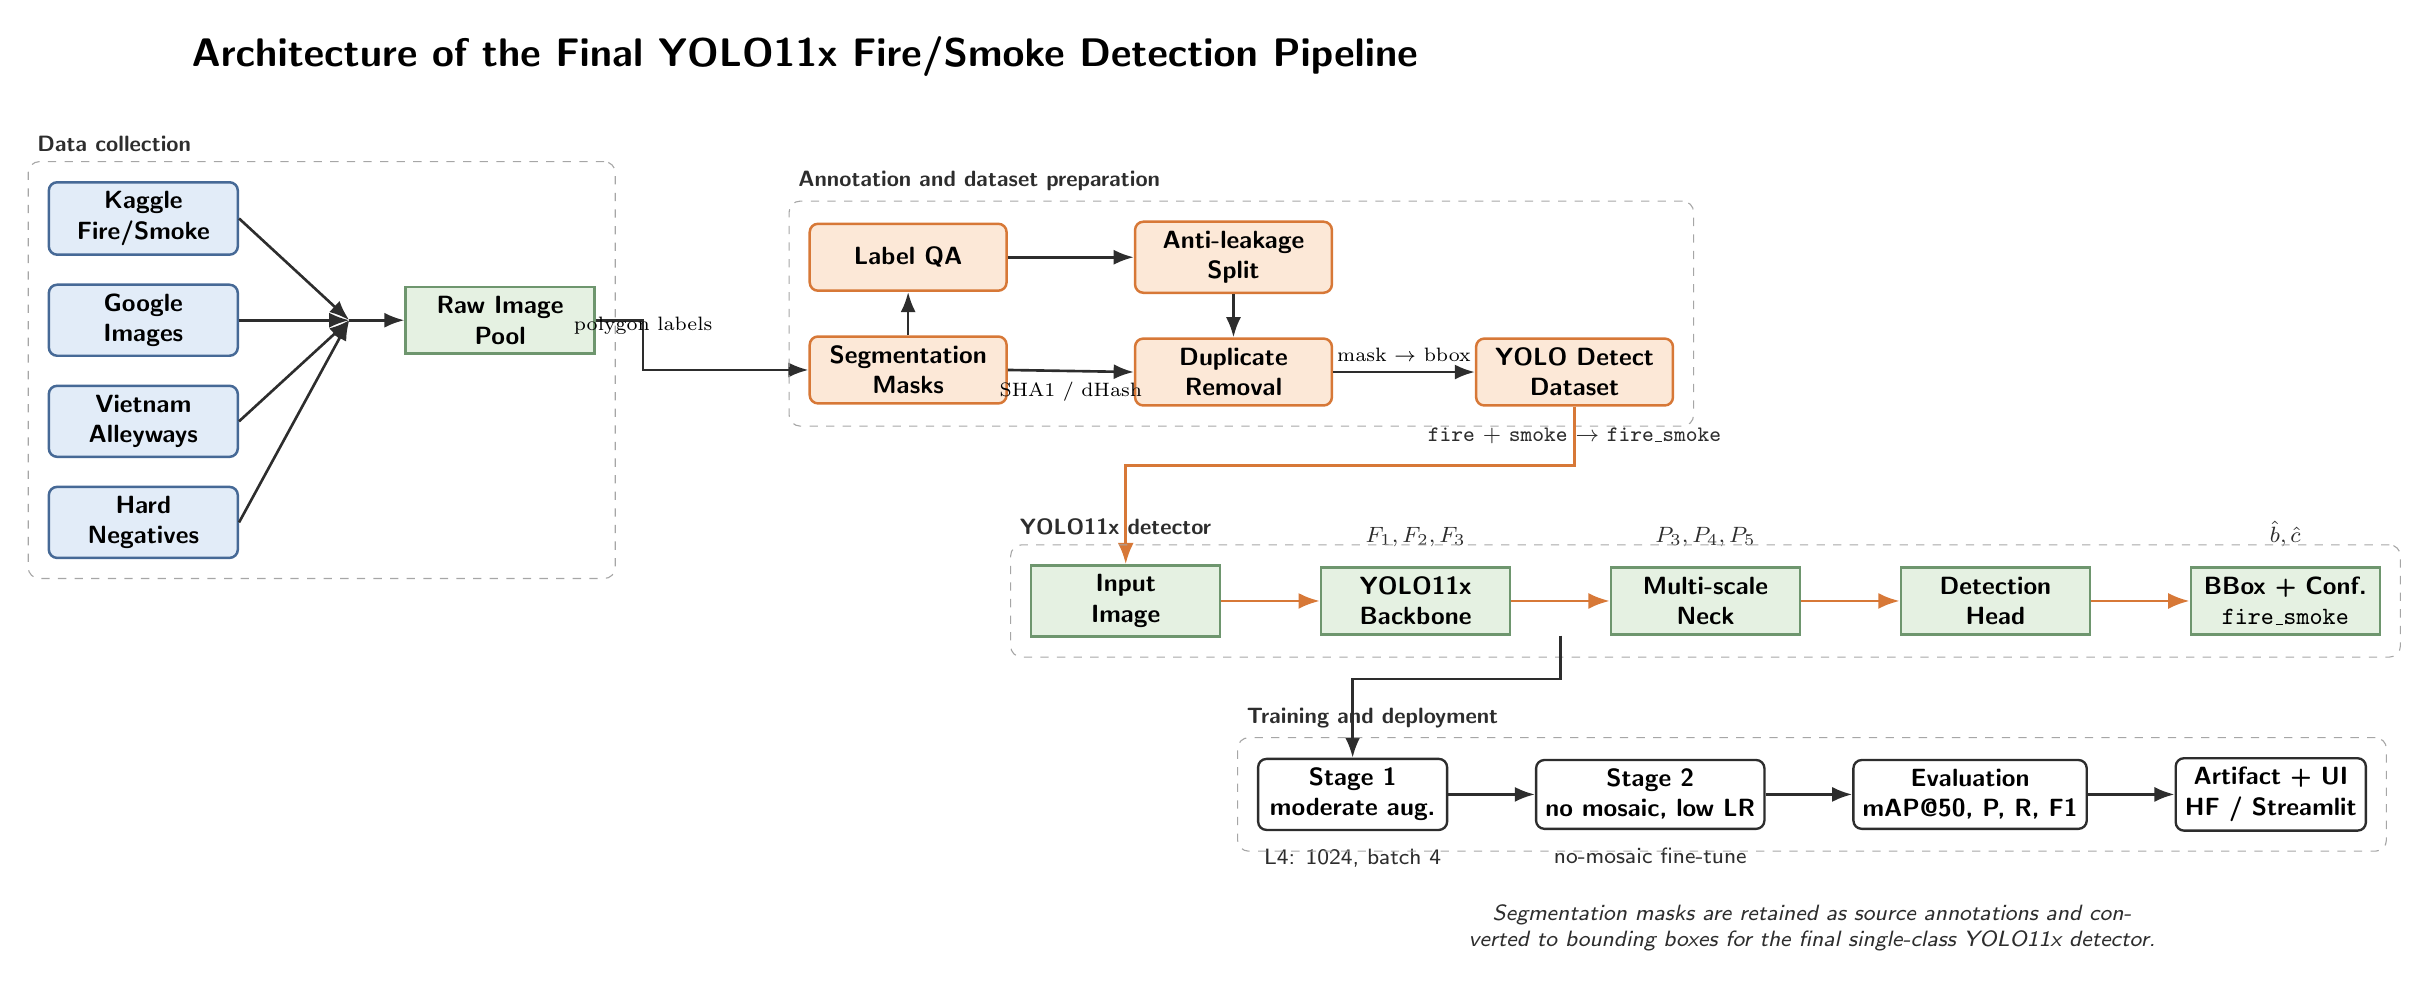
\begin{tikzpicture}[
    font=\sffamily,
    >=Latex,
    node distance=1.0cm and 1.2cm,
    data/.style={
        rectangle,
        rounded corners=3pt,
        draw=paperblue,
        fill=softblue,
        line width=0.9pt,
        minimum width=2.4cm,
        minimum height=0.85cm,
        align=center,
        font=\sffamily\small\bfseries
    },
    process/.style={
        rectangle,
        rounded corners=3pt,
        draw=paperorange,
        fill=softorange,
        line width=0.9pt,
        minimum width=2.5cm,
        minimum height=0.85cm,
        align=center,
        font=\sffamily\small\bfseries
    },
    model/.style={
        rectangle,
        draw=papergreen,
        fill=softgreen,
        line width=0.9pt,
        minimum width=2.4cm,
        minimum height=0.85cm,
        align=center,
        font=\sffamily\small\bfseries
    },
    metric/.style={
        rectangle,
        rounded corners=3pt,
        draw=darkgray,
        fill=white,
        line width=0.85pt,
        minimum width=2.4cm,
        minimum height=0.82cm,
        align=center,
        font=\sffamily\small\bfseries
    },
    arrow/.style={
        ->,
        line width=0.95pt,
        draw=darkgray
    },
    oarrow/.style={
        ->,
        line width=1.05pt,
        draw=paperorange
    },
    archlabel/.style={
        font=\sffamily\footnotesize,
        text=darkgray,
        align=center
    },
    grouplabel/.style={
        font=\sffamily\footnotesize\bfseries,
        text=darkgray
    },
    groupbox/.style={
        draw=gray!70,
        dashed,
        rounded corners=4pt,
        inner sep=7pt
    }
]

\node[font=\sffamily\bfseries\Large, align=center] (title)
at (0,0) {Architecture of the Final YOLO11x Fire/Smoke Detection Pipeline};

\node[data, below=1.2cm of title, xshift=-8.4cm] (kaggle) {Kaggle\\Fire/Smoke};
\node[data, below=0.35cm of kaggle] (google) {Google\\Images};
\node[data, below=0.35cm of google] (vietnam) {Vietnam\\Alleyways};
\node[data, below=0.35cm of vietnam] (hardneg) {Hard\\Negatives};

\node[model, right=2.1cm of google] (rawpool) {Raw Image\\Pool};

\coordinate (mergepoint) at ($(rawpool.west)+(-0.7,0)$);

\draw[arrow] (kaggle.east) -- (mergepoint);
\draw[arrow] (google.east) -- (mergepoint);
\draw[arrow] (vietnam.east) -- (mergepoint);
\draw[arrow] (hardneg.east) -- (mergepoint);
\draw[arrow] (mergepoint) -- (rawpool.west);

\node[groupbox, fit=(kaggle)(google)(vietnam)(hardneg)(rawpool)] (g1) {};
\node[grouplabel, anchor=south west] at (g1.north west) {Data collection};

\node[process, right=2.7cm of rawpool, yshift=0.8cm] (qa) {Label QA};
\node[process, below=0.55cm of qa] (segmask) {Segmentation\\Masks};
\node[process, right=1.6cm of qa] (split) {Anti-leakage\\Split};
\node[process, below=0.55cm of split] (dedup) {Duplicate\\Removal};
\node[process, right=1.8cm of dedup] (detectset) {YOLO Detect\\Dataset};

\draw[arrow] (rawpool.east) -- ++(0.6,0) |- node[pos=0.25, above, font=\scriptsize] {polygon labels} (segmask.west);
\draw[arrow] (segmask.north) -- (qa.south);
\draw[arrow] (qa.east) -- (split.west);
\draw[arrow] (split.south) -- (dedup.north);
\draw[arrow] (segmask.east) -- node[midway, below, font=\scriptsize] {SHA1 / dHash} (dedup.west);
\draw[arrow] (dedup.east) -- node[midway, above, font=\scriptsize] {mask $\rightarrow$ bbox} (detectset.west);

\node[archlabel, below=0.15cm of detectset] {\texttt{fire} + \texttt{smoke} $\rightarrow$ \texttt{fire\_smoke}};

\node[groupbox, fit=(qa)(segmask)(split)(dedup)(detectset)] (g2) {};
\node[grouplabel, anchor=south west] at (g2.north west) {Annotation and dataset preparation};

\node[model, below=2.0cm of detectset, xshift=-5.7cm] (inputimg) {Input\\Image};
\node[model, right=1.25cm of inputimg] (backbone) {YOLO11x\\Backbone};
\node[model, right=1.25cm of backbone] (neck) {Multi-scale\\Neck};
\node[model, right=1.25cm of neck] (head) {Detection\\Head};
\node[model, right=1.25cm of head] (output) {BBox + Conf.\\\texttt{fire\_smoke}};

\draw[oarrow] (inputimg.east) -- (backbone.west);
\draw[oarrow] (backbone.east) -- (neck.west);
\draw[oarrow] (neck.east) -- (head.west);
\draw[oarrow] (head.east) -- (output.west);

\draw[oarrow] (detectset.south) -- ++(0,-0.75) -| (inputimg.north);

\node[archlabel, above=0.12cm of backbone] {$F_1,F_2,F_3$};
\node[archlabel, above=0.12cm of neck] {$P_3,P_4,P_5$};
\node[archlabel, above=0.12cm of output] {$\hat{b},\hat{c}$};

\node[groupbox, fit=(inputimg)(backbone)(neck)(head)(output)] (g3) {};
\node[grouplabel, anchor=south west] at (g3.north west) {YOLO11x detector};

\node[metric, below=1.55cm of backbone, xshift=-0.8cm] (stage1) {Stage 1\\moderate aug.};
\node[metric, right=1.1cm of stage1] (stage2) {Stage 2\\no mosaic, low LR};
\node[metric, right=1.1cm of stage2] (eval) {Evaluation\\mAP@50, P, R, F1};
\node[metric, right=1.1cm of eval] (deploy) {Artifact + UI\\HF / Streamlit};

\draw[arrow] (stage1.east) -- (stage2.west);
\draw[arrow] (stage2.east) -- (eval.west);
\draw[arrow] (eval.east) -- (deploy.west);

\coordinate (detmid) at ($(backbone.south)!0.5!(neck.south)$);
\draw[arrow] (detmid) -- ++(0,-0.55) -| (stage1.north);

\node[archlabel, below=0.10cm of stage1] {L4: 1024, batch 4};
\node[archlabel, below=0.10cm of stage2] {no-mosaic fine-tune};

\node[groupbox, fit=(stage1)(stage2)(eval)(deploy)] (g4) {};
\node[grouplabel, anchor=south west] at (g4.north west) {Training and deployment};

\node[
    archlabel,
    below=0.55cm of g4,
    text width=10.8cm,
    font=\sffamily\footnotesize\itshape
] {
Segmentation masks are retained as source annotations and converted to
bounding boxes for the final single-class YOLO11x detector.
};

\end{tikzpicture}%
}
\caption{Final YOLO11x detection architecture and training pipeline.}
\label{fig:yolo11-arch}
\end{figure}

\section{Stage 1: Main Training}
Stage 1 initializes from \code{yolo11x.pt}. It trains on the sliced training dataset and evaluates on full validation/test images. Its role is to produce a strong baseline checkpoint.

\begin{table}[H]
\centering
\caption{Stage 1 training configuration}
\label{tab:stage1-config}
\begin{tabular}{lr}
\toprule
\textbf{Parameter} & \textbf{Value} \\
\midrule
Model & YOLO11x detect \\
Image size & 1024 \\
Epochs & 180 \\
Batch size & 4 \\
Optimizer & AdamW \\
Initial learning rate & 0.0005 \\
Scheduler & Cosine LR \\
Warmup & 4 epochs \\
Mosaic & 0.40 \\
MixUp & 0.02 \\
Scale & 0.35 \\
\bottomrule
\end{tabular}
\end{table}

\section{Stage 2: Fine-Tuning}
Stage 2 starts from the Stage 1 best checkpoint and disables mosaic/mixup. This encourages the model to adapt to real full-image distributions rather than synthetic mosaic compositions.

The observed improvement is small. Stage 1 reaches mAP@50 \(=0.445\), while Stage 2 reaches mAP@50 \(=0.454\), an absolute gain of only \(0.009\). The best Stage 2 checkpoint appears at epoch 7 out of the planned 60 epochs, suggesting early plateau. Therefore, Stage 2 should be interpreted as a minor refinement rather than a major modeling breakthrough. It may still be useful because it slightly improves mAP@50:95 and stabilizes no-mosaic behavior, but the current evidence is not strong enough to claim that the fine-tuning design is optimal.

This also suggests two follow-up experiments:

\begin{enumerate}
    \item compare Stage 2 against simply selecting the Stage 1 checkpoint with threshold tuning;
    \item sweep fine-tuning learning rates and shorter epoch schedules, because the current setup may be spending unnecessary compute after early convergence.
\end{enumerate}

\begin{table}[H]
\centering
\caption{Stage 2 fine-tuning configuration}
\label{tab:stage2-config}
\begin{tabular}{lr}
\toprule
\textbf{Parameter} & \textbf{Value} \\
\midrule
Initial weights & Stage 1 best checkpoint \\
Image size & 1024 \\
Epochs & 60 \\
Batch size & 4 \\
Learning rate & 0.00008 \\
Warmup & 1 epoch \\
Mosaic & 0.0 \\
MixUp & 0.0 \\
Scale & 0.20 \\
\bottomrule
\end{tabular}
\end{table}

\section{Training Results by Stage}
The Stage 2 checkpoint improves validation mAP slightly, but the model plateaus around mAP@50 \(=0.45\). Table~\ref{tab:stage-best} summarizes the best validation metrics.

\begin{table}[H]
\centering
\caption{Best validation metrics of Stage 1 and Stage 2}
\label{tab:stage-best}
\begin{tabular}{lrrrrr}
\toprule
\textbf{Stage} & \textbf{Best Epoch} & \textbf{Precision} & \textbf{Recall} & \textbf{mAP@50} & \textbf{mAP@50:95} \\
\midrule
Stage 1 & 97 & 0.578 & 0.432 & 0.445 & 0.253 \\
Stage 2 & 7 & 0.582 & 0.430 & 0.454 & 0.262 \\
\bottomrule
\end{tabular}
\end{table}

\begin{figure}[H]
\centering
\safeincludegraphics[width=0.82\textwidth]{figures/stage1_stage2_training/stage1_stage2_best_metrics.png}
\caption{Comparison of best Stage 1 and Stage 2 metrics.}
\label{fig:stage-best}
\end{figure}

\begin{figure}[H]
\centering
\safeincludegraphics[width=0.82\textwidth]{figures/stage1_stage2_training/stage1_stage2_map_comparison.png}
\caption{Stage 1 and Stage 2 mAP comparison.}
\label{fig:stage-map}
\end{figure}

\begin{figure}[H]
\centering
\safeincludegraphics[width=0.86\textwidth]{figures/stage1_stage2_training/stage1_training_curves.png}
\caption{Stage 1 training curves.}
\label{fig:stage1-curves}
\end{figure}

\begin{figure}[H]
\centering
\safeincludegraphics[width=0.86\textwidth]{figures/stage1_stage2_training/stage2_training_curves.png}
\caption{Stage 2 training curves.}
\label{fig:stage2-curves}
\end{figure}

\section{Compute Infrastructure and Cost}
The main experiments were run on rented NVIDIA L4 GPU resources. The approximate experimental cost was \(1{,}000{,}000\) VND. This is important because the report is not based on a trivial notebook run: the compute budget produced real model checkpoints, training curves, validation metrics, and error-analysis artifacts.

At the same time, GPU cost does not guarantee high mAP. For fire and smoke detection, model capacity is only one part of the problem. Label noise, hard negatives, small objects, duplicate leakage, and inference post-processing can dominate the final result. Therefore, the cost should be interpreted as the cost of a serious experiment and diagnosis, not as proof that the model must be deployment-ready.

% ===================== CHAPTER 6 =====================
\chapter{Evaluation and Error Analysis}
\section{Evaluation Metrics}
The final model is evaluated as a one-class detector. The main metrics are precision, recall, F1-score, mAP@50, and mAP@50:95:
\[
    \mathrm{Precision}=\frac{TP}{TP+FP}, \qquad
    \mathrm{Recall}=\frac{TP}{TP+FN},
\]
\[
    \mathrm{F1}=\frac{2\cdot \mathrm{Precision}\cdot \mathrm{Recall}}{\mathrm{Precision}+\mathrm{Recall}}.
\]

\section{Validation Per-Group Analysis}
Overall mAP hides group-specific weaknesses. Table~\ref{tab:group-valid} therefore reports per-group validation metrics using the Stage 2 checkpoint.

\begin{table}[H]
\centering
\small
\caption{Per-group validation error analysis}
\label{tab:group-valid}
\begin{tabularx}{\textwidth}{p{0.22\textwidth}rrrrrY}
\toprule
\textbf{Group} & \textbf{Images} & \textbf{GT} & \textbf{Precision} & \textbf{Recall} & \textbf{mAP@50} & \textbf{Interpretation} \\
\midrule
g01 positive\_standard & 527 & 1,506 & 0.551 & 0.410 & 0.426 & Main bottleneck due to low recall in the largest group. \\
g02 alley\_context & 42 & 105 & 0.690 & 0.476 & 0.566 & Better than g01, but sample size is small. \\
g03 hard\_negative & 19 & 0 & N/A & N/A & N/A & Requires false-positive analysis instead of mAP. \\
g04 sahi\_small\_objects & 20 & 108 & 0.865 & 0.714 & 0.760 & Slicing helps small objects, but localization remains weak at high IoU. \\
g05 ambient\_null & 233 & 0 & N/A & N/A & N/A & Requires false-positive analysis instead of mAP. \\
\bottomrule
\end{tabularx}
\end{table}

The validation results show that small objects are not the only issue. In fact, \code{g04} has the highest validation mAP@50. The major limitation is \code{g01}, where many positive standard scenes are still missed. This suggests that additional label QA and positive data diversity are necessary.

\section{Full-Image Test Evaluation}
The standard test benchmark evaluates the Stage 2 checkpoint on the original full-image test split at image size 1024. This is the most comparable setting to validation because both use the normal YOLO validation protocol rather than a custom slicing and merging pipeline. Ultralytics removed two duplicate labels from one test image during evaluation, so the full-image test contains 1,467 valid evaluated instances.

\begin{table}[H]
\centering
\footnotesize
\caption{Full-image test evaluation with the Stage 2 checkpoint}
\label{tab:full-image-test}
\begin{tabularx}{\textwidth}{p{0.31\textwidth}rrrrrr}
\toprule
\textbf{Group} & \textbf{Images} & \textbf{GT} & \textbf{P} & \textbf{R} & \textbf{mAP50} & \textbf{mAP50-95} \\
\midrule
Overall & 733 & 1,467 & 0.552 & 0.430 & 0.421 & 0.240 \\
g01 positive\_standard & 452 & 1,243 & 0.547 & 0.422 & 0.413 & 0.246 \\
g02 alley\_context & 42 & 132 & 0.660 & 0.477 & 0.561 & 0.346 \\
g03 hard\_negative & 19 & 0 & N/A & N/A & N/A & N/A \\
g04 sahi\_small\_objects & 20 & 92 & 0.770 & 0.543 & 0.511 & 0.182 \\
g05 ambient\_null & 200 & 0 & N/A & N/A & N/A & N/A \\
\bottomrule
\end{tabularx}
\end{table}

The full-image test shows that \code{g01} remains the largest source of missed positives. \code{g02} is the strongest positive test group, while \code{g04} confirms that the detector can still recover many small objects under normal full-frame inference. Because \code{g03} and \code{g05} contain no positive labels, their quality should be measured by false positives per image rather than by mAP.

\begin{figure}[htbp]
\centering
\safeincludegraphics[width=0.78\textwidth]{fullimg_eval/stage2_test/BoxPR_curve.png}
\caption{Full-image test precision-recall curve for the Stage 2 checkpoint.}
\label{fig:fullimg-pr}
\end{figure}

\begin{figure}[htbp]
\centering
\safeincludegraphics[width=0.62\textwidth]{fullimg_eval/stage2_test/confusion_matrix_normalized.png}
\caption{Normalized confusion matrix from the full-image test run.}
\label{fig:fullimg-confusion}
\end{figure}

The full-image test result changes the interpretation of the experiment. Validation mAP@50 \(=0.454\) and full-image test mAP@50 \(=0.421\) are reasonably close, so the model is not collapsing purely because of test-set distribution shift. The much lower sliced result should therefore be treated as an inference-protocol problem until further threshold and NMS sweeps prove otherwise.

\section{Sliced Inference Ablation}
The project also evaluates the Stage 2 checkpoint with sliced inference on the same test split. This protocol uses image size 1024, slice size 768, overlap 0.25, includes full-image prediction, and reports precision/recall at confidence 0.25.

This experiment is useful as an ablation, not as the main test result. Compared with the full-image mAP@50 of \(0.421\), sliced inference reaches only \(0.152\). The result shows that the current slicing, merging, and reporting thresholds are harmful in their present configuration, especially for recall.

\begin{footnotesize}
\begin{longtable}{lrrrrrrr}
\caption{Sliced inference evaluation on the test split}\label{tab:sliced-test}\\
\toprule
\textbf{Group} & \textbf{Images} & \textbf{GT} & \textbf{mAP@50} & \textbf{TP} & \textbf{FP} & \textbf{FN} & \textbf{Recall@0.25} \\
\midrule
\endfirsthead
\toprule
\textbf{Group} & \textbf{Images} & \textbf{GT} & \textbf{mAP@50} & \textbf{TP} & \textbf{FP} & \textbf{FN} & \textbf{Recall@0.25} \\
\midrule
\endhead
Overall & 733 & 1,469 & 0.152 & 210 & 292 & 1,259 & 0.143 \\
g01 & 452 & 1,245 & 0.202 & 176 & 151 & 1,069 & 0.141 \\
g02 & 42 & 132 & 0.252 & 27 & 35 & 105 & 0.205 \\
g03 & 19 & 0 & N/A & 0 & 6 & 0 & N/A \\
g04 & 20 & 92 & 0.110 & 7 & 2 & 85 & 0.076 \\
g05 & 200 & 0 & N/A & 0 & 98 & 0 & N/A \\
\bottomrule
\end{longtable}
\end{footnotesize}

\begin{figure}[H]
\centering
\safeincludegraphics[width=0.82\textwidth]{sliced_eval/stage2_test/sliced_pr_curve_iou50.png}
\caption{Sliced test precision-recall curve at IoU 0.50.}
\label{fig:sliced-pr}
\end{figure}

\begin{figure}[H]
\centering
\safeincludegraphics[width=0.86\textwidth]{sliced_eval/stage2_test/samples/g01_000103_sliced_pred.jpg}
\caption{Sliced inference prediction example from g01.}
\label{fig:sliced-sample-1}
\end{figure}

\begin{figure}[H]
\centering
\safeincludegraphics[width=0.86\textwidth]{sliced_eval/stage2_test/samples/g01_000287_sliced_pred.jpg}
\caption{Sliced inference prediction example with difficult localization.}
\label{fig:sliced-sample-2}
\end{figure}

\section{Interpreting the Low Metrics}
The results are below the original target, but the conclusion should be precise. The current model is not a failed experiment; it is a useful diagnostic experiment. There are three reasons.

\begin{enumerate}
    \item \textbf{Full-image and sliced tests measure different protocols.} Stage 2 validation reaches mAP@50 \(=0.454\), while the full-image test reaches mAP@50 \(=0.421\). This is a moderate and credible drop. The much lower sliced mAP@50 \(=0.152\) points to slicing, merging, and thresholding as likely causes, but a confidence/NMS sweep is still required before assigning exact responsibility.
    \item \textbf{The dataset is deliberately difficult and leakage-controlled.} Removing near-duplicates and preserving hard negatives can lower the metric compared with an easier leaked benchmark, but it makes the evaluation more honest.
    \item \textbf{The error analysis points to actionable fixes.} The main bottlenecks are false negatives in \code{g01}, low recall after thresholding/merging slices, and false alarms in ambient null scenes.
\end{enumerate}

\section{Critical Experimental Gaps}
\subsection{Full-Image Baseline Added, Ablations Still Missing}
The standard full-image test baseline has now been added, which fixes the largest comparability problem in the earlier analysis. The remaining experimental gap is systematic ablation. A stronger evaluation should still repeat the comparison under controlled threshold and NMS settings:

\begin{enumerate}
    \item keep full-image YOLO validation as the official test benchmark;
    \item run sliced inference using the same checkpoint and test split;
    \item sweep report confidence, tile confidence, merge IoU, and NMS settings;
    \item report per-group precision, recall, mAP, and false positives per image.
\end{enumerate}

Only this sequence can prove whether slicing improves small-object detection or damages recall through merging and thresholding.

\subsection{g04 Small-Object Protocol Gap}
The \code{g04 sahi\_small\_objects} result is still important, but the full-image test makes the issue clearer. On validation, \code{g04} achieves mAP@50 \(=0.760\) and recall \(=0.714\). On full-image test evaluation, \code{g04} remains usable with mAP@50 \(=0.511\) and recall \(=0.543\). In sliced test evaluation, however, \code{g04} recall@0.25 drops to \(0.076\). This means the model can detect some small objects, while the current sliced inference protocol is failing to preserve them.

Several hypotheses are possible:

\begin{itemize}
    \item the validation and test \code{g04} subsets may differ in object scale or visual difficulty;
    \item mAP on full-image validation and recall@0.25 on sliced inference are different measurements;
    \item sliced inference may generate candidate boxes that are removed or merged incorrectly;
    \item the threshold \(0.25\) may be too high for small objects;
    \item the validation subset may be too small to represent true small-object performance.
\end{itemize}

The report therefore treats this as a protocol gap rather than a solved error. A confidence sweep and a full-image-vs-sliced comparison on \code{g04} are required before concluding that SAHI helps or hurts small-object detection.

\subsection{No Confidence/NMS Sweep}
The current sliced test uses a fixed report confidence of \(0.25\), tile IoU \(0.70\), and merge IoU \(0.55\). Because no sweep is available, the claim that post-processing is the cause of the gap remains a hypothesis. A stronger experiment would evaluate:

\[
    conf \in \{0.05, 0.10, 0.15, 0.20, 0.25, 0.30, 0.35\}
\]
and multiple merge-IoU/NMS values. The expected output should be a table or curve showing the precision--recall trade-off, especially for \code{g04} and negative groups.

\section{Main Error Categories}
\subsection{False Negatives in Positive Standard Scenes}
\code{g01 positive\_standard} contributes most of the missed objects. This suggests that the model still fails on common positive cases, not only on rare edge cases. Possible causes include label inconsistency, visually subtle smoke, small flame regions, and large intra-class variation.

\subsection{Hard Negative Confusion}
Hard negatives and ambient null frames remain essential. The test sliced protocol produced false positives in \code{g03} and \code{g05}. In a fire alerting system, even a modest false positive rate is harmful because repeated false alarms reduce user trust.

\subsection{Sliced Inference Post-Processing}
Sliced inference was expected to help small objects, but the current configuration produces low recall. The likely issue is not simply model capacity; it may be the interaction among low candidate threshold (\code{conf=0.001}), merge IoU, NMS, and final report confidence. However, this remains unproven until a sweep is run. A threshold/NMS sweep is required before this can be considered deployment-ready.

% ===================== CHAPTER 7 =====================
\chapter{Discussion}
\section{Why the Project Still Has Academic Value}
The final metric does not reach the target, but the project demonstrates a rigorous Data Mining process. A superficial report could hide low performance by using duplicated data, easy images, or only overall mAP. This report instead shows the difficult parts: manual labeling, data cleaning, negative sampling, group-wise evaluation, and post-processing diagnosis.

From an academic perspective, this is valuable because it produces falsifiable conclusions:

\begin{itemize}
    \item The dataset after deduplication is harder but more realistic.
    \item Stage 2 fine-tuning improves validation mAP only slightly.
    \item Small-object validation is not the sole bottleneck.
    \item Full-image test evaluation is the main benchmark, while sliced inference currently reduces recall.
    \item More GPU compute alone is unlikely to solve the problem without better data and post-processing.
\end{itemize}

\section{Recommended Improvement Plan}
The next iteration should prioritize data and evaluation rather than blindly training more stages.

\begin{enumerate}
    \item \textbf{Keep full-image test as the official benchmark:} Use the Stage 2 checkpoint result on the original full-image test split as the primary score.
    \item \textbf{Compare full-image and sliced inference systematically:} Run both protocols on the same split, same checkpoint, and same metric script where possible.
    \item \textbf{QA the largest false-negative group:} Recheck \code{g01} labels and inspect images where the model misses objects.
    \item \textbf{Expand hard negatives:} Add more lamps, reflections, sunset, welding, haze, and night-scene backgrounds.
    \item \textbf{Run confidence/NMS sweeps:} Evaluate \code{report\_conf} from 0.05 to 0.35 and adjust merge IoU for sliced inference.
    \item \textbf{Quantify annotation quality:} Estimate inter-annotator agreement and label error rate on a sampled subset.
    \item \textbf{Active learning:} Run inference on unlabeled images and select uncertain samples for annotation.
    \item \textbf{Repeat L4 experiments after data fixes:} Reuse the same L4 protocol after label QA and post-processing sweeps so improvements remain comparable to the reported experiments.
\end{enumerate}

% ===================== CHAPTER 8 =====================
\chapter{Conclusion}
This project built a serious Computer Vision and Data Mining pipeline for fire and smoke detection. The strongest contributions are not limited to the final YOLO11x checkpoint. The project collected multi-source data, created segmentation annotations from image-only sources, designed meaningful data groups, removed near-duplicates, prevented leakage through source-level splitting, generated data audit artifacts, trained on rented NVIDIA L4 compute, packaged the Stage 1/2 checkpoints on Hugging Face, implemented a local Streamlit inference interface, and performed group-wise and sliced inference error analysis.

The best Stage 2 validation result achieved mAP@50 \(=0.454\), below the initial target of mAP@50 \(\geq 0.70\). The full-image test benchmark achieved Precision \(=0.552\), Recall \(=0.430\), mAP@50 \(=0.421\), and mAP@50:95 \(=0.240\). This is the main test result. The sliced test ablation reached mAP@50 \(=0.152\) and recall@0.25 \(=0.143\), showing that the current sliced inference configuration is not ready for deployment.

The main lesson is that fire/smoke detection is a data-centric problem. Compute is necessary, and nearly \(1{,}000{,}000\) VND was spent on rented NVIDIA L4 experiments, but GPU time alone cannot overcome noisy labels, missing annotation-quality statistics, or untuned inference protocols. The correct next step is not merely to train longer, but to improve labels, add targeted hard negatives, sweep threshold/NMS settings, and use active learning to close the recall gap.

\section*{Final Statement}
\addcontentsline{toc}{section}{Final Statement}
Although the final metric is not high, the project is valuable as a rigorous experimental pipeline. It honestly documents the work required to build a dataset, train a modern detector, pay for real GPU experiments, package a checkpoint artifact, provide a usable inference test UI, and diagnose why the model underperforms. The remaining weaknesses are now explicit: missing confidence/NMS sweeps, missing quantitative annotation-quality measurement, background false-positive measurement, and a small-object sliced-inference protocol gap. This makes the report stronger than a simple high-score demo because it shows both engineering capability and scientific honesty.

\end{document}
